\section{Handling Variable-Length Sequences}

So far we have mainly focused on models that handle \textbf{input and output of fixed size}. For example, in a convolutional neural network (CNN), we transform an input in the form of a matrix (image) into an output in the form of a vector (labels). However, the community has developed models that can handle variable-length structures, more specifically sequences, such as text, which is a sequence of strings.

Recurrent Neural Networks (RNNs) are flexible tools that can perform many different tasks, which can be classified as follows:

\begin{figure}[!htbp]
    \centering
    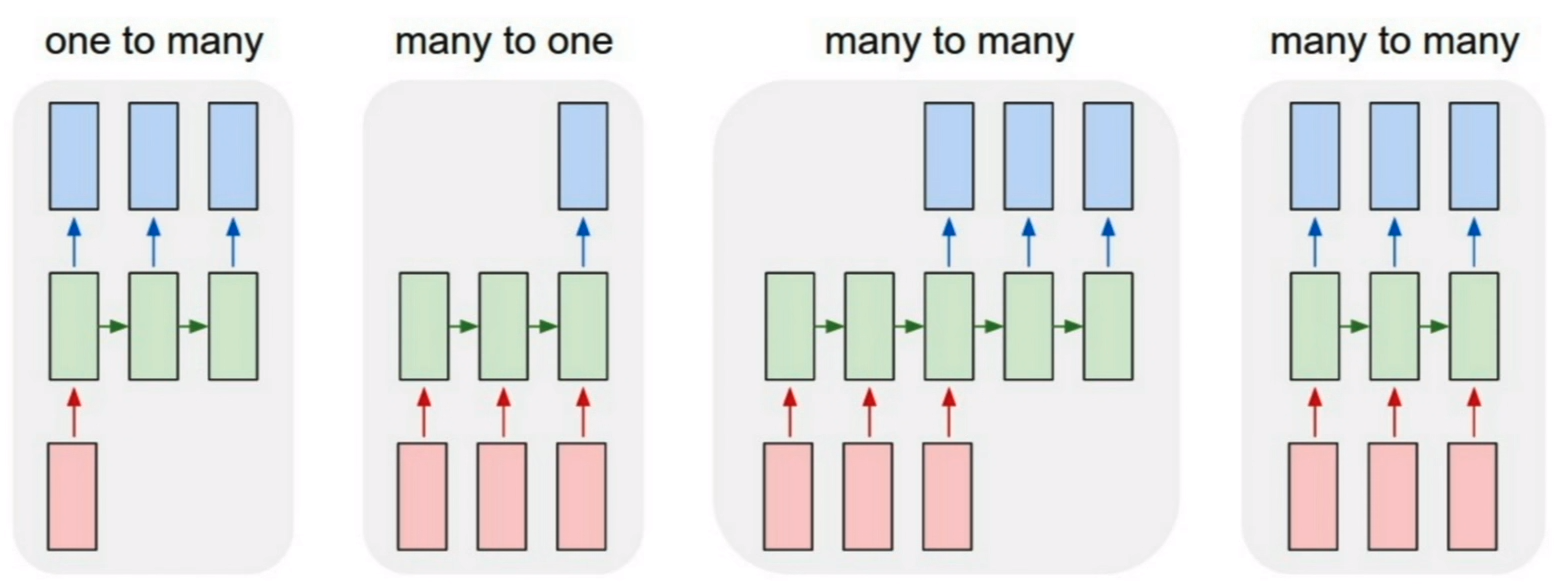
\includegraphics[width=\textwidth]{tikz/chapter6 - Types of RNN Models.png}
    \caption{{\color{red}\colorbox{pink}{Tikz TO-DO: the second before the first one}} Diagrams of RNN Models}
\end{figure}

\subsection{Multiple2Single: Sentiment Analysis}

In the sentiment analysis, the model must classify a product, restaurant, or any other item as positive, neutral, or negative based on the reviews received. In this scenario, we provide the neural network with inputs of varying sizes. Each word is transformed into a \textbf{hidden representation that reflects the context and propagates through subsequent words}, as these words are not independent of each other. This propagation occurs unidirectionally, similar to a feedforward neural network. However, the main difference is that instead of mapping a single input to an output of fixed size, the model takes multiple inputs and produces a single label. Predictions are typically made about the last hidden state, which should include the context of previous words.

\subsection{Single2Multiple: Image Captioning}

In image captioning, the network is fed a fixed input (an image), but the output will have a variable length, since we want to produce a sentence describing the content of the image. In this case, the latent representation of the image obtained from a CNN is \textbf{combined with the latent representations of the words to model the dependencies between them}. This approach allows a single input to be mapped to multiple outputs, generating several words that describe the image.

\subsection{Multiple2Multiple: Machine Translation}

In machine translation, the task is to translate a sentence from one language to another. This problem involves both multiple inputs and multiple outputs. Each word in the input sentence is mapped to a hidden representation that takes into account the context of the preceding words. The neural network uses these representations to generate the translated sentence, word by word, \textbf{maintaining sequential dependencies between words}. This allows the model to produce an accurate translation that reflects the meaning of the original sentence.

\section{Vanilla RNN}

Recurrent neural networks are, in essence, \textbf{neural networks with cycles}.

The Vanilla RNN, introduced in \href{https://www.sciencedirect.com/science/article/pii/036402139090002E}{"Finding structure in time" (Jeffrey L. Elman)}, has a \textbf{recurrent design} in that it performs the same parametric function for each input ($x_t$, each marked with a timestep), while the output ($h_t$, the hidden representation marked with the corresponding timestep) depends on the previous computation ($h_{t-1}$). After producing the output, this is \textbf{used to generate the hidden representation of the next RNN cell} ($h_{t+1}$). To make a decision ($y_t$), a linear layer can be applied to the end of a cell, considering both the current input and the output learned from the previous input.

There are two types of representations for an RNN: the \textbf{Folded} representation, which is synthetic, and the \textbf{Unfolded} representation, which provides a more explicit description of the computations. Below is the architecture of the network in both representations:

\begin{figure}[!htbp]
    \centering
    \includegraphics[width = 0.9\linewidth]{tikz/chapter6 - RNN Architecture.pdf}
    \caption{{\color{red}\colorbox{pink}{Tikz To Refine}} RNN Architecture}
\end{figure}

The structure of an RNN cell, as shown in the figure above, has two inputs ($x_t$ and $h_{t-1}$) and can be represented mathematically as follows:

$$
h_t = f_W(x_t,h_{t-1}) = \text{tanh} \ W \begin{pmatrix}
x_t \\
h_{t-1}
\end{pmatrix} = \text{tanh}(W_xx_t + W_hh_{t-1})
$$

In this equation, $h_t$ represents the hidden state at time $t$, $x_t$ is the input at time $t$, $h_{t-1}$ is the previous hidden state, $W_x$ and $W_h$ are the weights associated with the current input and previous hidden state respectively. The function $\text{tanh}$ provides nonlinearity to the network (\textit{Using hyperbolic tangent is understandable given that the paper is from the 1990s, a time when the use of it was common}). During training, $W$ weights are learned through the optimization process. For the prediction:
$$
y_t = \text{softmax}(W_y h_t + b_y)
$$
A peculiar aspect of RNNs is the \textbf{sharing of weights among different timesteps}: the weights $W_x$, $W_h$ and $W_y$ are shared between different timestep iterations, allowing the model to capture \textbf{sequential dependencies within the data}.

So, the main differences between an RNN and an FNN include the sharing of weights between timesteps, the use of backpropagation variation for training (in which we need to sum the contributions along the entire sequence) and the presence of three different sets of weights: $W_x$, $W_h$ and $W_y$. In addition, \textbf{the problem of gradient vanishing is more severe} in RNNs than in feedforward networks, mainly because of the hyperbolic tangent function used as the activation function. Also, backpropagation through time can be computationally expensive for a large number of timesteps.


\subsection{Truncated BPTT (Backpropagation Through Time)}


To solve the problems described above, we use the Truncated BPTT algorithm, which is a more efficient technique when dealing with long sequences. It was introduced as a Ph.D. thesis in \href{https://www.cs.utoronto.ca/~ilya/pubs/ilya_sutskever_phd_thesis.pdf}{"Training Recurrent Neural Networks" (Ilya Sutskever)}.

The idea of Truncated BPTT is to simplify this process. Instead of running the entire sequence through the network, we divide it into \textbf{smaller blocks of fixed length}. Each block is treated as a separate training unit. In this way, the network does not have to work with the whole sequence at once, but only with small chunks at a time, making training more efficient.

After presenting a block to the network, \textbf{backpropagation is performed only for a limited number of backward time steps}, rather than traversing the entire length of the sequence. This means that the network does not have to keep track of information too far back in time, reducing the computational cost of training.

To control how far back in time to go during backpropagation, we use two parameters, $k_1$ and $k_2$. The first, $k_1$, determines the \textbf{length of the blocks} into which we divide the sequence, while $k_2$ defines the \textbf{number of time steps} over which to perform backpropagation within each block. The Truncated BPTT algorithm can be schematized as follows:

\begin{algorithm}
\renewcommand\thealgorithm{}
\caption{}
\begin{algorithmic}[1]
\STATE Present a sequence of $k_1$ timesteps of input and output pairs to the network.
\STATE Unroll the network then calculate and accumulate errors across $k_2$ timesteps.
\STATE Roll-up the network and update weights.
\STATE Repeat the process.
\end{algorithmic}
\end{algorithm}
Adjusting $k_1$ and $k_2$ allows us to balance the training speed and the network's ability to capture long-range time dependencies.

\section{Long Short-Term Memory (LSTM)}

It has been recognized that the classical RNN suffers from an inefficient design in its individual cell, as efforts to improve learning have not produced significant improvements in the vanishing gradient problem due to inherent limitations in the cell design. To solve this problem, LSTM was introduced. The architecture was first presented in this article: \href{https://deeplearning.cs.cmu.edu/F23/document/readings/LSTM.pdf}{"Long Short-term Memory" (Sepp Hochreiter)}.

The LSTM cell not only produces the hidden state $h_t$, but adds another component called \textbf{Memory Cell} ($c_t$), which is responsible for maintaining and deleting information, based on the input context. This means that \textbf{some of the previous information must be remembered, some must be forgotten, and some new information must be added to memory}. Here is the design of the cell:

\begin{figure}[!htbp]
    \centering
    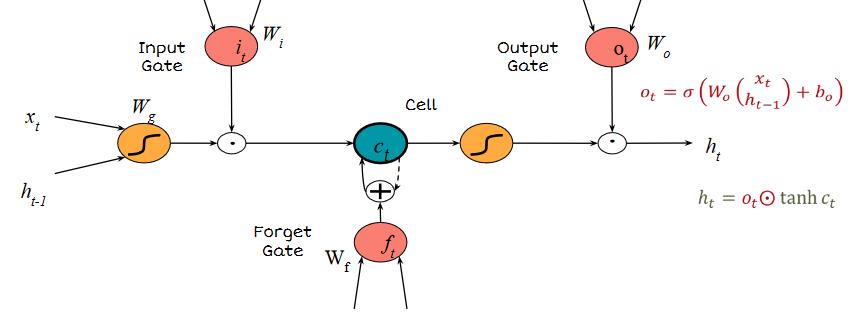
\includegraphics[width=\linewidth]{tikz/chapter6 - LSTM.png}
    \caption{{\color{red}\colorbox{pink}{Tikz TO-DO}} LSTM Cell Structure}
\end{figure}

As you can see, within an LSTM cell, there are three different parametric components, called \textbf{Gate}. Let's explore them in detail.

\begin{remark}{mybluee}{mybluee!20}
\textbf{Input Gate}: can allow the input signal ($x_t$ and $h_{t-1}$) to alter the state of the memory cell or block it.

Its output $i_t$ is computed by the sigmoid function applied to the input $x_t$ and the preceding dependency $h_{t-1}$, and is associated with its own parameters $W_i$:
$$ i_t = \sigma(W_i
\begin{pmatrix}
x_t \\
h_{t-1}
\end{pmatrix} + b_i)
$$

$i_t$ is used as a trade-off between the information passing through the current input ($x_t$ and $h_{t-1}$) and the information encoded by the previous cell ($c_{t-1}$).
\end{remark}

\begin{remark}{myred}{myred!20}
\textbf{Forget Gate}: can modulate the self-recurrent connection of the memory cell, allowing the cell to remember or forget its previous state as needed.

Its output $f_t$ is computed by the sigmoid function applied to the input $x_t$ and the previous dependency $h_{t-1}$, and is associated with its own parameters $W_f$:
$$ f_t = \sigma(W_f
\begin{pmatrix}
x_t \\
h_{t-1}
\end{pmatrix} + b_f)
$$
\end{remark}


\begin{remark}{accent}{accent!5}
\textbf{Memory Cell Calculation} is a combination of the previous two gates:
$$c_t = \textcolor{myred}{f_t} \odot c_{t-1} + \textcolor{mybluee}{i_t} \odot g_t $$

We can interpret the equation as follows:
\begin{itemize}
    \item \( \textcolor{myred}{f_t} \odot c_{t-1}\): The forget gate decides how much of the cell's previous state \( c_{t-1} \) should be forgotten or retained for the next state \( c_t \).
    
    \item \( \textcolor{mybluee}{i_t} \odot g_t \): This determines how much of the new information \( g_t \), i.e., the value of the input modulation, should be added to the state of the cell \( c_t \).
\end{itemize}
In short, \textbf{\textcolor{myred}{the forget gate modulates how much of the previous state to retain}}, while \textbf{\textcolor{myblue}{the input gate modulates how much of the new information is to be added to the cell state}}.
\end{remark}

\begin{remark}{mygreen}{mygreen!20}
\textbf{Output Gate}: can allow the state of the memory cell ($c_t$) to have an effect on other neurons, thus affecting the output of the LSTM unit ($h_t$).

First, a sigmoid layer decides which parts of the cell state ($c_t$) the model is going to produce as output (associated with its parameters $W_o$):
$$ o_t = \sigma(W_o
\begin{pmatrix}
x_t \\
h_{t-1}
\end{pmatrix} + b_o)
$$
\end{remark}

\begin{remark}{accent}{accent!5}
To \textbf{Calculate the Output} of the cell, a tanh layer is used on the state of the memory cell to shrink values between -1 and 1, which are then multiplied by the output of the sigmoid gate:
$$h_t = \textcolor{mygreen}{o_t} \odot \text{tanh}(c_t) $$
\end{remark}

It is important to note that although there are many nonlinearity functions, the calculations to update the value of the cell ($c_t$) are \textbf{linear}, so the gradient flow from $c_t$ to $c_{t-1}$ involves only \textbf{backpropagation through addition and element-by-element multiplication}, not multiplication of matrices or nonlinear functions.

We can also formulate a (\textit{beautiful}) compact version of everything we have seen, summarizing the formulas in:
$$
\setlength{\arraycolsep}{5pt}
\renewcommand{\arraystretch}{0.95}
\begin{pmatrix}
g_t \\
\textcolor{mybluee}{i_t} \\
\textcolor{myred}{f_t} \\
\textcolor{mygreen}{o_t} 
\end{pmatrix} = 
\begin{pmatrix}
\text{tanh} \\
\sigma \\
\sigma \\
\sigma 
\end{pmatrix}
\begin{pmatrix}
W_g \\
\textcolor{mybluee}{W_i} \\
\textcolor{myred}{W_f} \\
\textcolor{mygreen}{W_o}
\end{pmatrix}
\begin{pmatrix}
x_t \\
h_{t-1}
\end{pmatrix}
$$
$$c_t = \textcolor{myred}{f_t} \odot c_{t-1} + \textcolor{mybluee}{i_t} \odot g_t $$
$$h_t = \textcolor{mygreen}{o_t} \odot \text{tanh}(c_t) $$

\section{Gated Recurrent Unit (GRU)}
As the community began to apply LSTM models to various tasks such as captioning, it became apparent that the network was overly complex. Thus, thanks to \href{https://arxiv.org/pdf/1406.1078}{"Learning Phrase Representations using RNN Encoder–Decoder
for Statistical Machine Translation" (Cho et al.)}, the GRU network was introduced to address this complexity by simplifying the LSTM cell by \textbf{removing one of its gates}. Despite having only two gates, the model is sufficiently resilient to the vanishing gradient problem. Moreover, the information flow is stored only in the hidden state $h_t$. Here is the architecture of a cell:

\begin{figure}[!htbp]
    \centering
    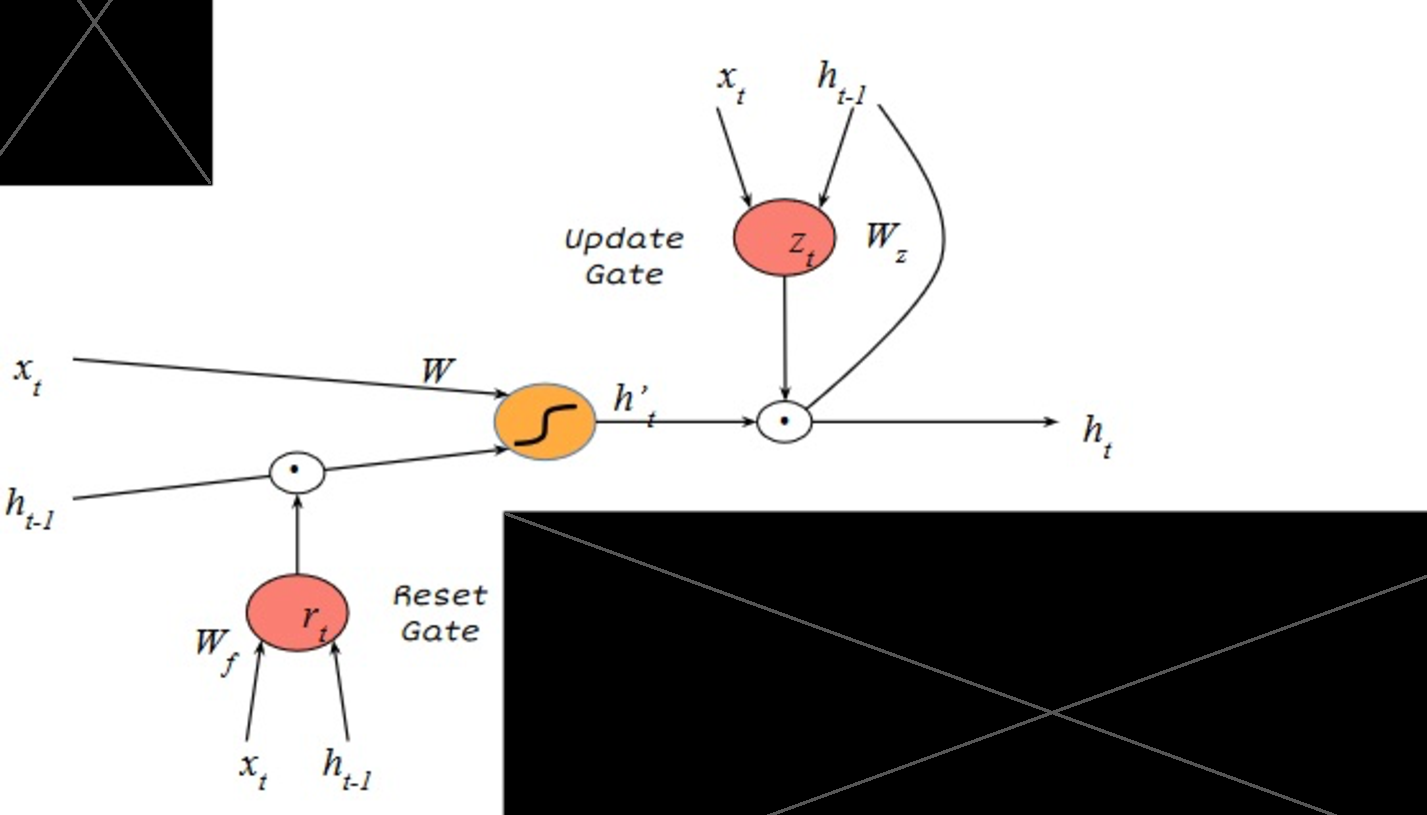
\includegraphics[width=0.85\linewidth]{tikz/chapter6 - GRU.pdf}
    \caption{{\color{red}\colorbox{pink}{Tikz TO-DO}} GRU Cell Structure}
\end{figure}

As before, let's analyze together the gates used in the GRU model.

\begin{remark}{myorange}{myorange!20}
\textbf{Reset Gate}: used to decide how much of the passed information to forget.

The output $r_t$ is computed by the sigmoid function applied to the input $x_t$ and the previous hidden state $h_{t-1}$, and is associated with its own parameters $W_r$:
$$ r_t = \sigma(W_r
\begin{pmatrix}
x_t \\
h_{t-1}
\end{pmatrix} + b_t)
$$
\end{remark}

\begin{remark}{accent}{accent!5}
An important change in the design of the LSTM cell is that \textbf{the value of the input modulation is no longer based solely on the complete information from the previous hidden state} $h_{t-1}$, but instead on a "restricted stream" determined by $\textcolor{myorange}{r_t}$:

$$ h'_t = \text{tahn }W(
\begin{pmatrix}
x_t \\
\textcolor{myorange}{r_t} \odot h_{t-1}
\end{pmatrix})
$$
\end{remark}

\begin{remark}{myyellow!85!black}{myyellow!20}
\textbf{Update Gate}: helps the model determine how much of the past information (from previous time steps) needs to be transmitted to the future.

The output $z_t$ is computed by the sigmoid function applied to the input $x_t$ and the previous hidden state $h_{t-1}$, and is associated with its own parameters $W_z$:

$$ z_t = \sigma(W_z
\begin{pmatrix}
x_t \\
h_{t-1}
\end{pmatrix} + b_z)
$$
\end{remark}


\begin{remark}{accent}{accent!5}
The \textbf{Final Representation of the Hidden State} is calculated by an additional point product:

$$h_t = (1-\textcolor{myyellow!85!black}{z_t})\odot h_{t-1}+\textcolor{myyellow!85!black}{z_t} \odot h'_t$$
\end{remark}
